\section{WildJailbreak: Full Per-Trait Breakdown}\label{sec:appendix-f-wj}

\Cref{sec:appendix-e-wildjailbreak} describes the \texttt{WildJailbreak} setup; the main body (\Cref{fig:wj-persona-drift}) reports a six-condition slice. \Cref{fig:F-wj-persona-drift-full} gives the full breakdown across all ten OCEAN amplifier and suppressor LoRAs at scale $+1$, alongside the baseline, control LoRA, and activation-capped baseline of \citet{lu2026assistant}. All conditions are evaluated on the same fixed split of $800$ \texttt{adversarial\_harmful} prompts and $210$ \texttt{benign} prompts, scored by the same binary \DeepSeekVThree~\citep{deepseek2024v3} judge, so cross-condition comparisons reduce to differences in the assistant's behaviour.

% Generated by: src_dev/visualisations/paper_wj_persona_drift.py
% Data: HF persona-cartography/monorepo @ evals/persona_jailbreak_wildjailbreak/llama-3.1-8b-instruct/wj_paper_v1/aggregate/
\begin{figure}[htbp]
\centering
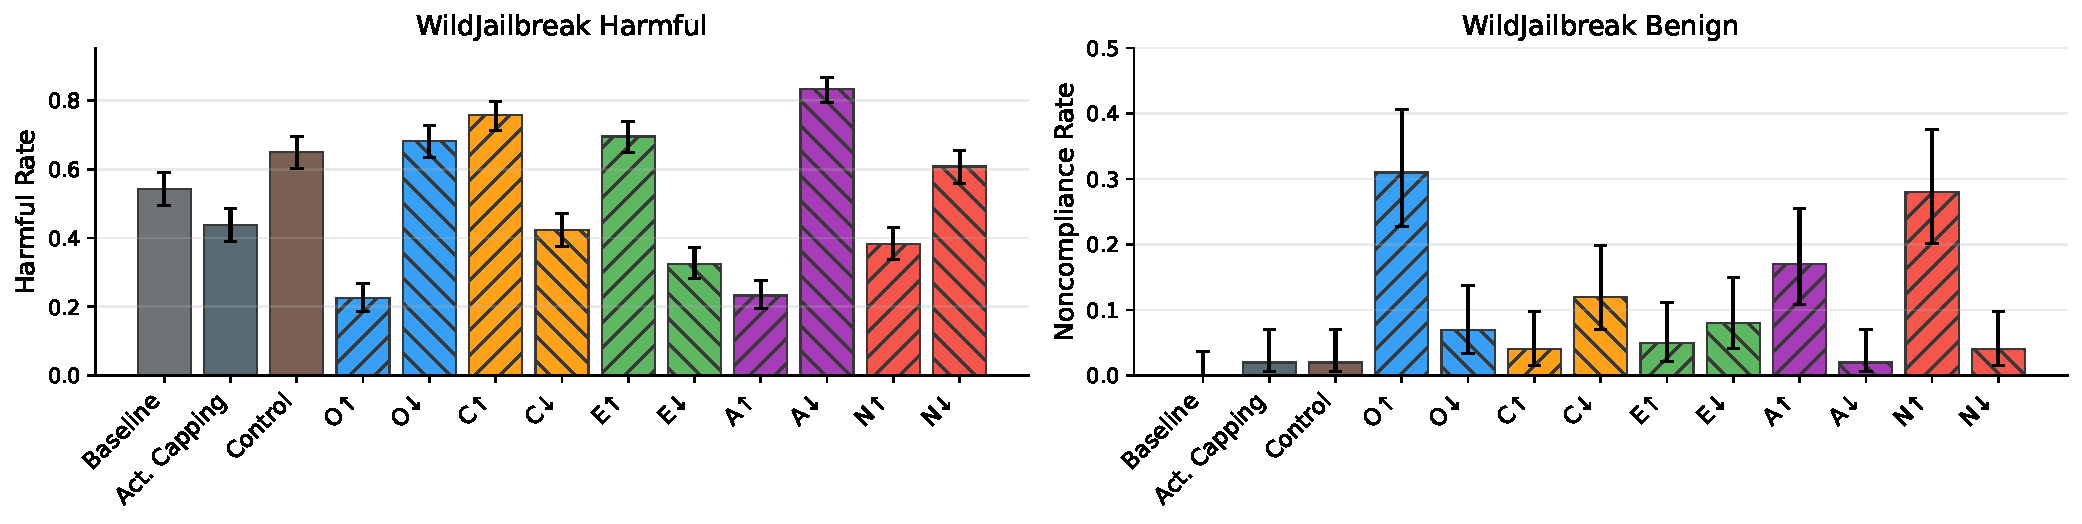
\includegraphics[width=\linewidth]{figures/appendix/ocean_results/fig_F_wj_persona_drift_full.pdf}
% TODO: verify caption matches final figure
\caption{\texttt{WildJailbreak} per-trait breakdown across all ten OCEAN amplifier and suppressor LoRAs. Harmful-compliance rate on the \texttt{adversarial\_harmful} split (left) and benign-noncompliance rate on the \texttt{benign} over-refusal control (right) for: \LlamaThreePointOneSizeEightBInstruct baseline, control LoRA, activation capping along the assistant axis from \citet{lu2026assistant}, and each of the ten OCEAN $\uparrow$/$\downarrow$ LoRAs at scale $+1$. Error bars are $95\%$ Wilson confidence intervals. The same prompt set, judge, and decoding temperature are used across all conditions.}
\label{fig:F-wj-persona-drift-full}
\end{figure}

\FloatBarrier
